\documentclass[11pt,a4paper]{article}

\usepackage[margin=22mm,headheight=15pt]{geometry}
\usepackage[T1]{fontenc}
\usepackage{lmodern}
\usepackage{microtype}
\usepackage{amsmath,amssymb}
\usepackage{siunitx}
\usepackage{booktabs}
\usepackage{graphicx}
\usepackage{float}
\usepackage{enumitem}
\usepackage{xcolor}
\usepackage{caption}
\usepackage{fancyhdr}
\usepackage[hidelinks]{hyperref}

\definecolor{navy}{HTML}{17365D}
\definecolor{lightblue}{HTML}{EAF1F8}
\definecolor{rulegray}{HTML}{B8C2CC}

\hypersetup{
  pdftitle={Saturation Temperature and Pressure Report 2026},
  pdfauthor={Aaron Taylor},
  pdfsubject={ENME 601 Thermodynamics Laboratory 1},
  pdfkeywords={saturation pressure, PT100, steam tables, thermodynamics}
}

\captionsetup{font=small,labelfont=bf,justification=centering}
\sisetup{round-mode=places,round-precision=2,detect-all}
\setlist[itemize]{leftmargin=6mm,itemsep=1.5pt,topsep=3pt}
\setlist[enumerate]{leftmargin=7mm,itemsep=2pt,topsep=3pt}
\setlength{\parindent}{0pt}
\setlength{\parskip}{5pt}
\setlength{\tabcolsep}{5pt}
\setlength{\emergencystretch}{1.5em}

\pagestyle{fancy}
\fancyhf{}
\fancyhead[L]{\small ENME 601 Thermodynamics}
\fancyhead[R]{\small Saturation Temperature and Pressure}
\fancyfoot[C]{\thepage}
\renewcommand{\headrulewidth}{0.4pt}

\newcommand{\sectionrule}{\vspace{-2pt}\color{rulegray}\hrule\color{black}\vspace{5pt}}
\newenvironment{evidencebox}{%
  \begin{center}\begin{minipage}{0.94\linewidth}\colorbox{lightblue}{\begin{minipage}{0.95\linewidth}\small\textbf{Evidence note.}\ }}%
  {\end{minipage}\end{minipage}\end{center}}

\begin{document}

\begin{center}
  {\LARGE\bfseries Saturation Temperature and Pressure Lab}\par
  \vspace{3mm}
  {\large Aaron Taylor --- 24232594}\par
  \vspace{1.5mm}
  {\large August 1, 2026}\par
\end{center}
\vspace{4mm}

\section*{Synopsis}
\sectionrule
The relationship between the saturation temperature and absolute pressure of
water was investigated using an Armfield TH3 saturation-pressure apparatus.
Nine equilibrium-stage readings were recorded between \SI{50}{\kilo\pascal} and
\SI{450}{\kilo\pascal} gauge pressure. Gauge pressures were converted to absolute
pressure using the measured atmospheric pressure of \SI{101.65}{\kilo\pascal},
and PT100 resistance readings were converted to temperature using the
laboratory calibration. The initial comparison graph used the experimental
points together with the pressure--temperature values stated directly in the
saturated-water pressure table. Linear interpolation was used later only to
find a theoretical temperature at each experimental absolute pressure for the
point-by-point error calculations.

Both datasets followed a smooth power relationship of the form
$T=AP^n$. The experimental fit was $T=37.633P^{0.2146}$, compared with
$T=31.019P^{0.2557}$ for the direct steam-table data. Experimental temperatures were
below the theoretical values at every point. Signed error changed from
$-1.21\%$ at \SI{151.65}{\kilo\pascal} absolute to $-6.47\%$ at
\SI{551.65}{\kilo\pascal} absolute, with a mean signed error of $-4.32\%$.
The growing negative deviation identifies a systematic effect rather than
random scatter, most plausibly incomplete thermal equilibrium, heat loss and
probe lag, residual non-condensable air, or uncertainty in the two-point
resistance calibration.

\section{Aim}
\sectionrule
To measure the relationship between the saturation temperature and absolute
pressure of water, model that relationship with a power law, and assess the
accuracy of the apparatus by comparison with published saturated-water data.

\section{Theory}
\sectionrule
At liquid--vapour equilibrium, water and saturated steam coexist at one
saturation temperature for a given absolute pressure. Increasing pressure
raises the saturation temperature and produces a smooth saturation curve in
temperature--pressure space.

The pressure sensor records gauge pressure, so atmospheric pressure must be
added:
\begin{equation}
  P_{\mathrm{abs}}=P_1+P_{\mathrm{atm}},
  \qquad P_{\mathrm{atm}}=\SI{101.65}{\kilo\pascal}.
  \label{eq:pressure}
\end{equation}

The PT100 conversion used the two calibration points recorded during the
laboratory:
\begin{equation}
  \alpha=\frac{R_2-R_1}{T_2-T_1}
  =\frac{138.7-109.0}{100-15}
  =\SI{0.34941}{\ohm\per\degreeCelsius},
  \label{eq:alpha}
\end{equation}
\begin{equation}
  T_{\mathrm{exp}}=T_1+\frac{R-R_1}{\alpha}
  =15+\frac{R-109.0}{0.34941}.
  \label{eq:temperature}
\end{equation}

Over the measured range, the saturation relationship was represented by
\begin{equation}
  T_{\mathrm{sat}}=AP_{\mathrm{sat}}^n,
  \label{eq:power}
\end{equation}
where $A$ and $n$ were determined separately for the experimental dataset and
the values stated directly in the steam table. Interpolation was not used to
construct this comparison dataset.

The theoretical temperature at each experimental pressure was found by linear
interpolation:
\begin{equation}
  T_{\mathrm{th}}=T_a+
  \frac{P_{\mathrm{abs}}-P_a}{P_b-P_a}(T_b-T_a).
  \label{eq:interpolation}
\end{equation}
Signed percentage error was calculated as specified in the laboratory
instructions:
\begin{equation}
  \mathrm{Error}\ (\%)=
  \frac{T_{\mathrm{exp}}-T_{\mathrm{th}}}{T_{\mathrm{th}}}\times100.
  \label{eq:error}
\end{equation}

\section{Equipment}
\sectionrule
The equipment comprised an Armfield TH3 saturation-pressure apparatus with a
\SI{2.4}{\litre} boiler, sight glass, closed pipe loop, cartridge heaters,
control console, filling and pressure-relief valves, a PT100 resistance
thermometer, electronic and Bourdon pressure gauges, a barometer, and
de-ionised water.

\begin{figure}[H]
  \centering
  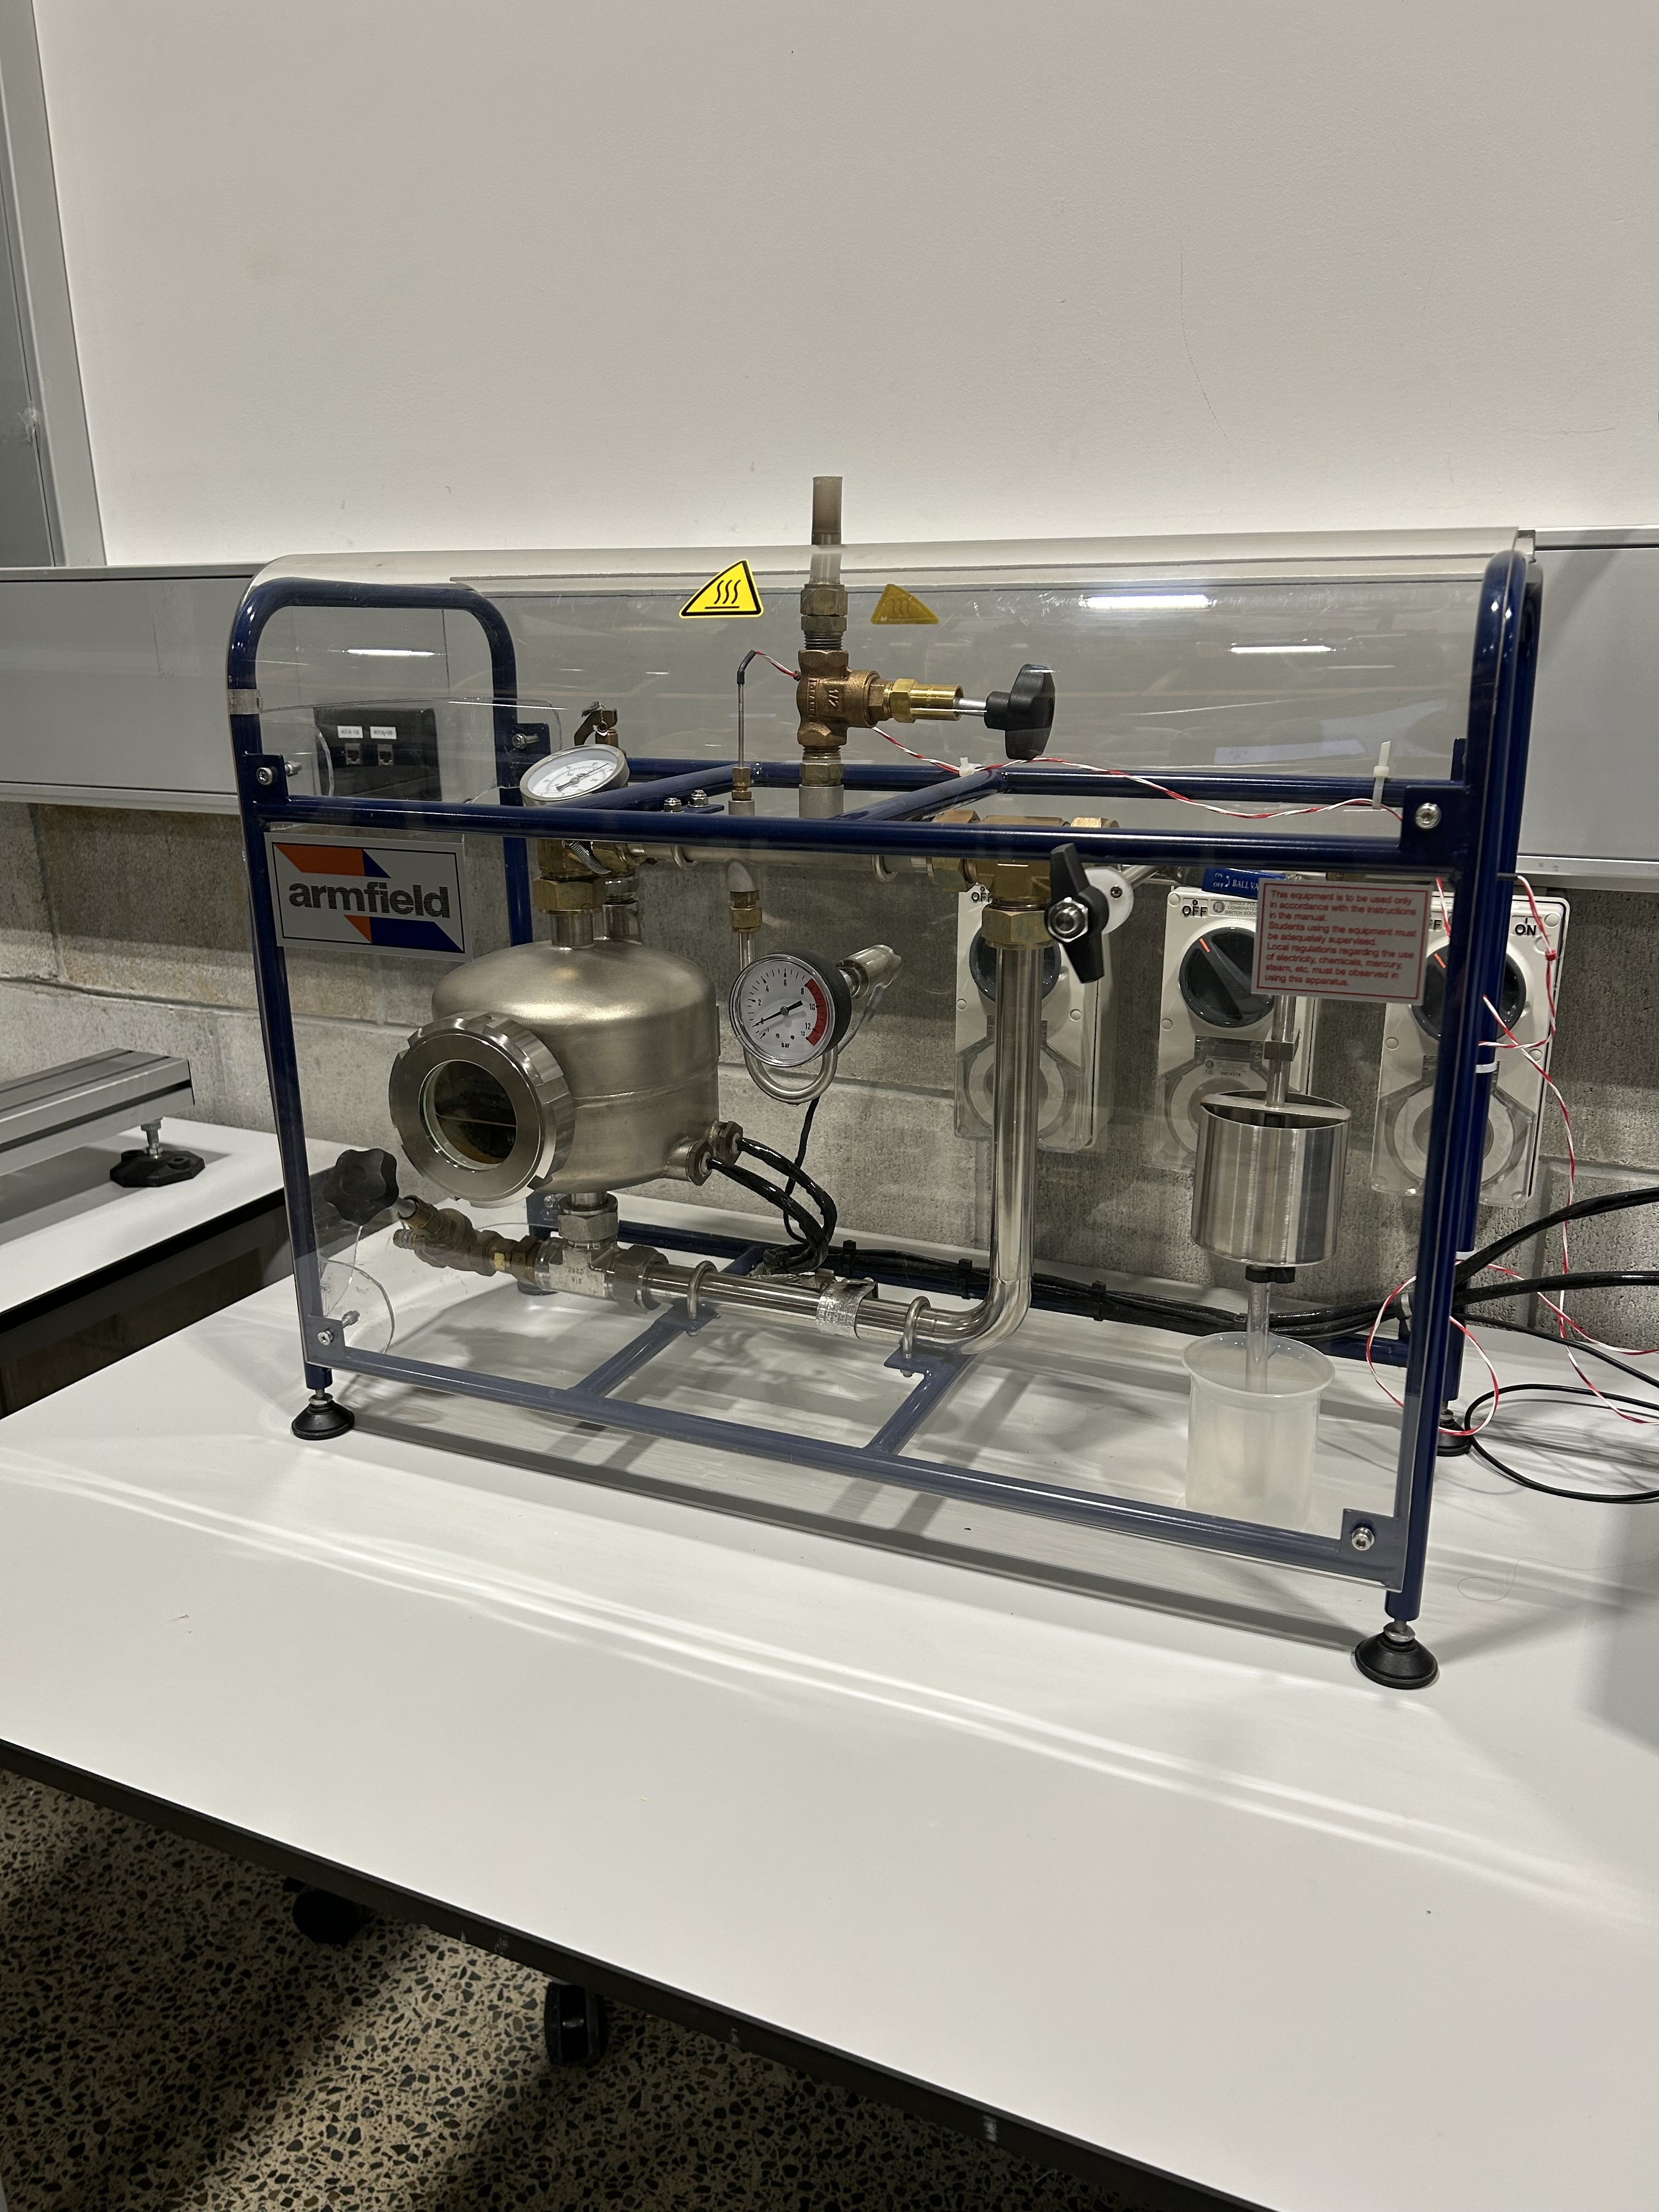
\includegraphics[width=0.90\textwidth,height=0.42\textheight,keepaspectratio]{Figure 1 - TH3 apparatus.jpeg}
  \caption{Armfield TH3 boiler and pipe loop used to produce and measure saturated
  steam. The photograph records the apparatus, pressure gauge, viewing port,
  valves and sensor wiring used in the 2026 experiment.}
  \label{fig:apparatus}
\end{figure}

\section{Method}
\sectionrule
\begin{enumerate}
  \item With the drain and isolating valves closed and console power off, the
        boiler was filled with de-ionised water to halfway up the sight glass
        while the filling-point valve remained open.
  \item The water was heated to vigorous boiling and steam was vented until the
        indication stabilised, purging air from the loop. The filling-point valve
        was then closed to form a constant-volume saturated mixture.
  \item Heater input was raised for approximately two minutes and then reduced.
        Readings were taken only after the PT100 indication stabilised.
  \item Gauge pressure and PT100 resistance were recorded at nine stages from
        \SI{50}{\kilo\pascal} to \SI{450}{\kilo\pascal} gauge pressure.
  \item Gauge pressures were converted to absolute pressure and resistances to
        experimental temperature. The experimental points and the values stated
        directly in Table A--5 were plotted on the same axes and fitted separately.
  \item For the error table only, theoretical saturation temperatures were
        interpolated from Table A--5 at each experimental absolute pressure.
        Temperature errors were then calculated for all nine points.
\end{enumerate}

\section{Results}
\sectionrule
\subsection{Atmospheric pressure}
The atmospheric pressure measured on the laboratory day was
\SI{101.65}{\kilo\pascal}. This value was added to every gauge-pressure reading
to obtain the absolute pressures reported below.

\subsection{Experimental and steam-table saturation curves}
Figure~\ref{fig:temperature} compares the experimental measurements with the
pressure--temperature pairs stated directly in Table A--5. The steam-table
markers are the published values at \SI{150}{\kilo\pascal},
\SI{175}{\kilo\pascal}, \SI{200}{\kilo\pascal} and the subsequent tabulated
pressures through \SI{600}{\kilo\pascal}; they were not interpolated to match the
experimental pressures. Each dataset was fitted independently to Equation~\ref{eq:power}.

\begin{figure}[H]
  \centering
  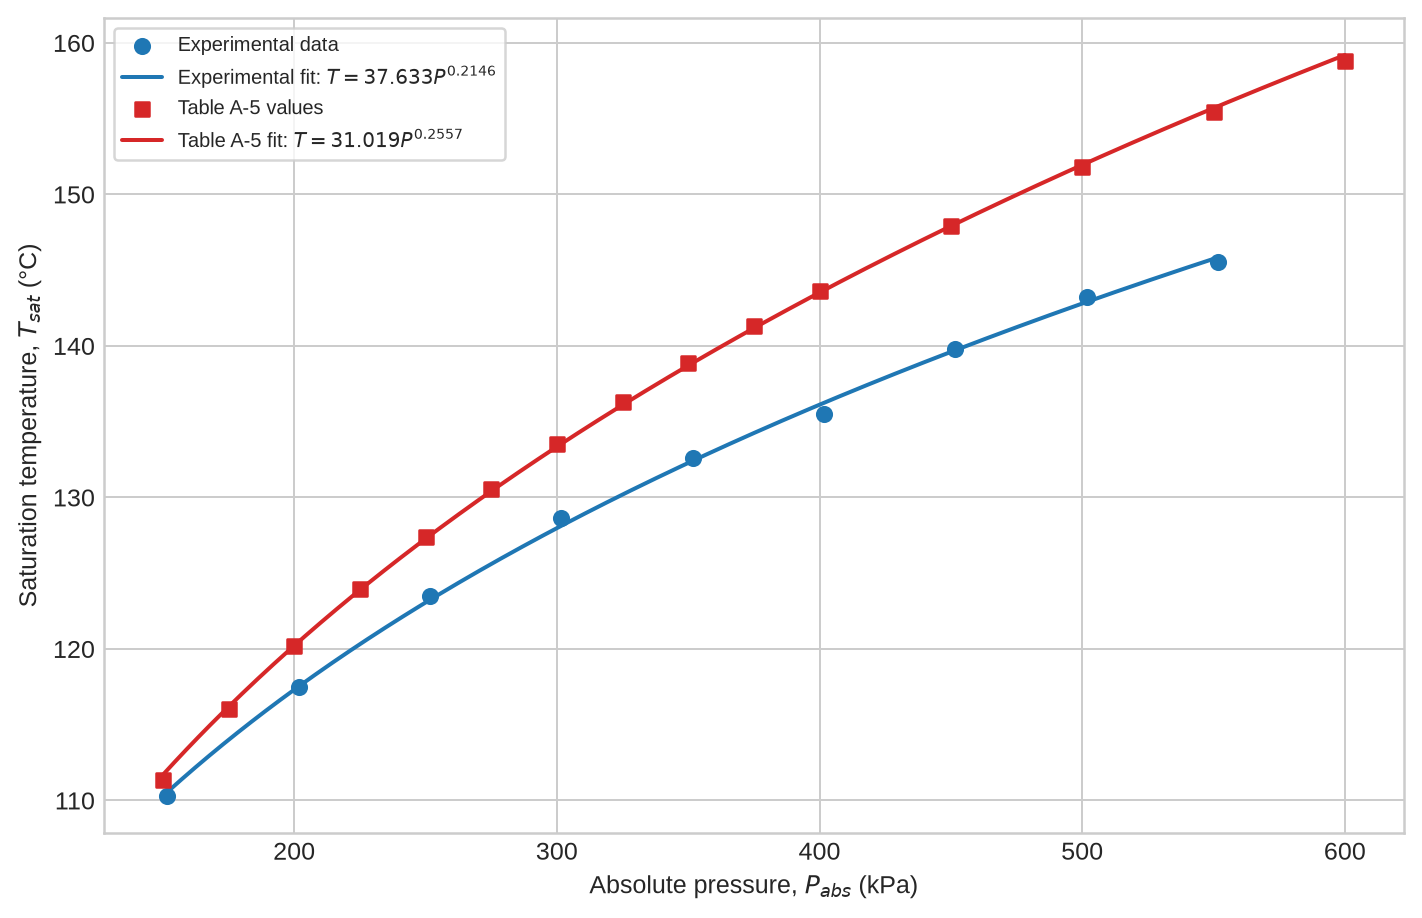
\includegraphics[width=0.91\textwidth]{Figure 2 v2 - Experimental and Table A5 values.png}
  \caption{Experimental PT100-derived temperatures and the saturation values
  stated directly in Table A--5, plotted against absolute pressure with separate
  power-law trendlines. No interpolated theoretical points are used in this graph.}
  \label{fig:temperature}
\end{figure}

\begin{table}[H]
  \centering
  \caption{Power-law fit parameters for $T=AP^n$.}
  \label{tab:fits}
  \begin{tabular}{lrrr}
    \toprule
    Dataset & $A$ & $n$ & $R^2$ \\
    \midrule
    Experimental measurements & 37.633 & 0.2146 & 0.99895 \\
    Direct Table A--5 values & 31.019 & 0.2557 & 0.99983 \\
    \bottomrule
  \end{tabular}
\end{table}

\subsection{Point-specific interpolation and error calculations}
Interpolation was then applied separately to determine $T_{\mathrm{th}}$ at each
experimental $P_{\mathrm{abs}}$. For the first reading,
$P_1=\SI{50.00}{\kilo\pascal}$ and $R=\SI{142.3}{\ohm}$:
\begin{align}
  P_{\mathrm{abs}} &= 50.00+101.65
  =\SI{151.65}{\kilo\pascal},\\
  T_{\mathrm{exp}} &= 15+\frac{142.3-109.0}{0.34941}
  =\SI{110.30}{\degreeCelsius}.
\end{align}
The pressure-table values enclosing \SI{151.65}{\kilo\pascal} are
\SI{111.35}{\degreeCelsius} at \SI{150}{\kilo\pascal} and
\SI{116.04}{\degreeCelsius} at \SI{175}{\kilo\pascal}. Therefore,
\begin{align}
  T_{\mathrm{th}}
    &=111.35+\frac{151.65-150}{175-150}(116.04-111.35)
      =\SI{111.66}{\degreeCelsius},\\
  \mathrm{Error}
    &=\frac{110.30-111.66}{111.66}\times100=-1.21\%.
\end{align}

\begin{table}[H]
  \centering
  \caption{Point-specific interpolated temperatures and corresponding errors.}
  \label{tab:results}
  \small
  \begin{tabular}{rrrrrr}
    \toprule
    $P_1$ & $P_{\mathrm{abs}}$ & $R$ & $T_{\mathrm{exp}}$ & $T_{\mathrm{th}}$ & Error \\
    (kPa gauge) & (kPa) & ($\Omega$) & ($^\circ$C) & ($^\circ$C) & (\%) \\
    \midrule
     50 & 151.65 & 142.3 & 110.30 & 111.66 & $-1.21$ \\
    100 & 201.65 & 144.8 & 117.46 & 120.46 & $-2.49$ \\
    150 & 251.65 & 146.9 & 123.47 & 127.62 & $-3.25$ \\
    200 & 301.65 & 148.7 & 128.62 & 133.70 & $-3.80$ \\
    250 & 351.65 & 150.1 & 132.63 & 139.02 & $-4.60$ \\
    300 & 401.65 & 151.1 & 135.49 & 143.75 & $-5.75$ \\
    350 & 451.65 & 152.6 & 139.78 & 148.03 & $-5.57$ \\
    400 & 501.65 & 153.8 & 143.22 & 151.95 & $-5.75$ \\
    450 & 551.65 & 154.6 & 145.51 & 155.57 & $-6.47$ \\
    \bottomrule
  \end{tabular}
\end{table}

\begin{figure}[H]
  \centering
  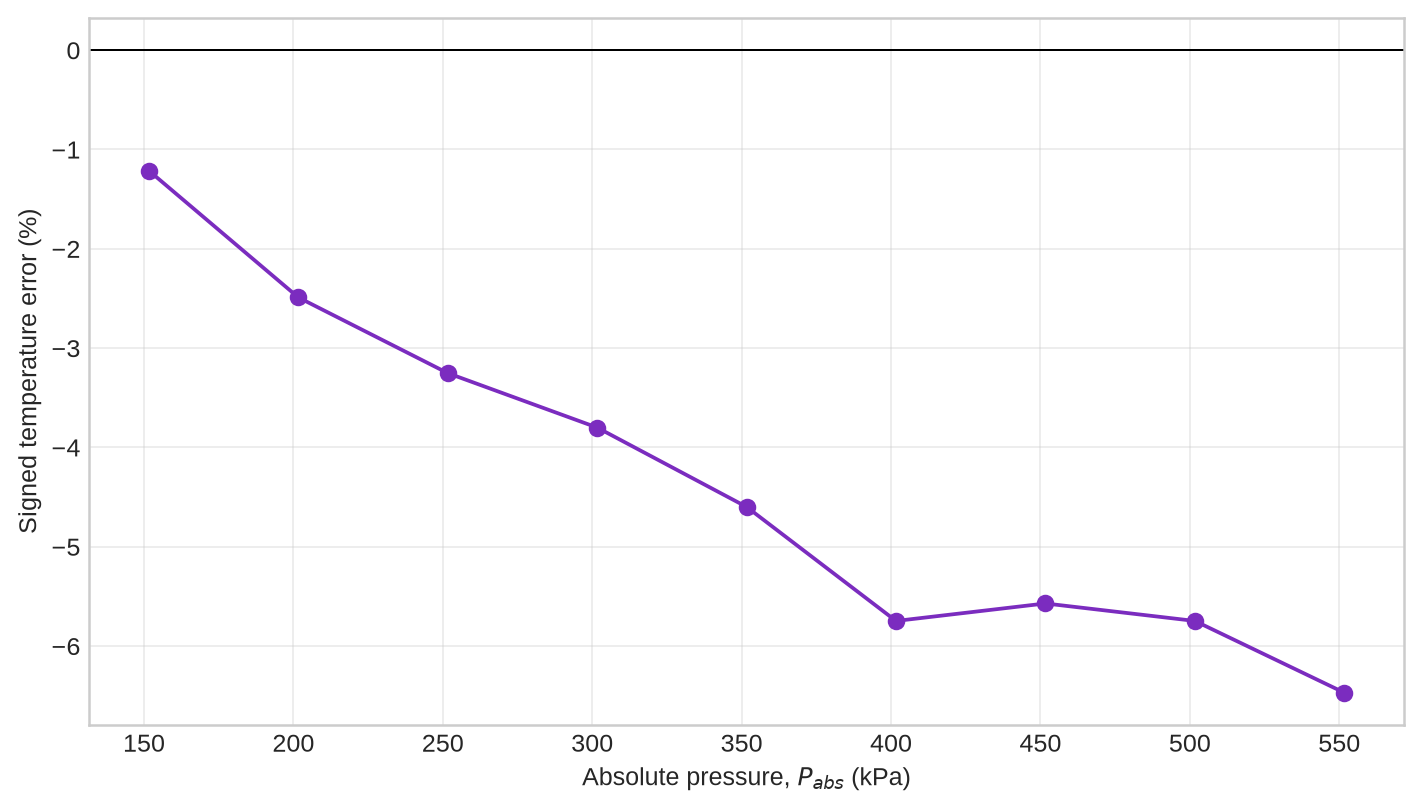
\includegraphics[width=0.90\textwidth]{Figure 3 - Error versus absolute pressure.png}
  \caption{Signed experimental temperature error relative to the point-specific
  interpolated saturation temperatures.}
  \label{fig:error}
\end{figure}

The mean signed error was $-4.32\%$, and the mean absolute error was $4.32\%$
because every experimental value was below its theoretical value. The maximum
absolute error was $6.47\%$ at \SI{551.65}{\kilo\pascal} absolute.

\section{Discussion}
\sectionrule
\subsection{Comparison of the saturation curves}
Both curves increased smoothly with absolute pressure, and both power-law fits
had $R^2>0.998$, confirming that the measurements captured the expected form of
the saturation relationship. However, the experimental curve became
progressively lower than the steam-table curve as pressure increased. The
mismatch was therefore systematic rather than the result of scattered readings.

\subsection{Accuracy and usefulness of the fitted equation}
The experimental exponent, $n=0.2146$, was lower than the direct-table fit of
$0.2557$. Consequently, the experimental equation predicts too little
temperature rise as pressure increases. It is useful as an empirical
description only within the measured range and for this apparatus calibration.
It should not replace the steam tables for design calculations or extrapolation.
The theoretical fit follows the reference data more closely and is the more
reliable compact approximation over this pressure interval.

\subsection{Error trend}
Error became generally more negative as pressure rose, changing from $-1.21\%$
to $-6.47\%$. A small improvement occurred at \SI{451.65}{\kilo\pascal}, but it
did not alter the overall trend. This pattern indicates a pressure-dependent
bias. Reporting only the mean error would conceal this behaviour; Figure
\ref{fig:error} therefore provides stronger evidence than a single average.

\subsection{Steam temperature, water temperature and thermal lag}
Liquid water and steam have the same saturation temperature only when both
phases are in thermodynamic equilibrium at the measured pressure. The PT100
measured steam in the upper pipework rather than liquid in the boiler. During
heating, energy must conduct through the fluid, metalwork and probe sheath before
the sensor reaches the steam temperature. Heat loss from the exposed loop can
also make the local probe temperature lower than the bulk saturation
temperature. If readings are taken before full stabilisation, both effects
produce a negative temperature error, particularly at higher heater input and
pressure.

\subsection{Likely sources of error}
\begin{itemize}
  \item \textbf{Residual air:} air remaining when the filling valve was closed
  contributes partial pressure. The sensor then measures steam pressure plus air
  pressure, while saturation temperature depends on steam partial pressure.
  This produces a measured temperature below the value expected from total pressure.
  \item \textbf{Thermal lag and insufficient stabilisation:} the increasingly
  negative error is consistent with the PT100 lagging the changing steam temperature.
  \item \textbf{Heat loss and temperature gradients:} the upper loop and sensor
  fittings lose heat to the room, so the local steam/probe temperature can be
  below the boiler saturation temperature.
  \item \textbf{Calibration uncertainty:} derived temperatures depend on the
  two-point linear conversion recorded on the whiteboard. Uncertainty in
  $R_1$, $T_1$, $R_2$ or sensor linearity affects every result systematically.
  \item \textbf{Pressure measurement:} pressure-sensor calibration, gauge
  resolution and the atmospheric-pressure reading affect every calculated
  absolute pressure.
  \item \textbf{Interpolation and rounding:} linear interpolation and recorded
  precision introduce smaller numerical errors, though these are insufficient
  to explain the observed trend.
\end{itemize}

The strongest improvements would be to purge the loop for longer, record only
after both resistance and pressure remain stable, use the PT100's certified
resistance--temperature relation or a traceable calibration, and repeat each
pressure point to quantify repeatability.

\section{Conclusion}
\sectionrule
The experiment reproduced the expected increase in water saturation temperature
with absolute pressure. The experimental data were smooth and fitted a power
law with $R^2=0.99895$, but they did not match the reference curve as closely as
their smoothness alone might suggest. Experimental temperatures were below the
interpolated steam-table values at all nine points, with a mean signed error of
$-4.32\%$ and a maximum absolute error of $6.47\%$. The increasing negative
error and lower experimental exponent identify a systematic measurement effect,
most likely associated with thermal lag, heat loss, residual air, or
resistance-calibration uncertainty. Steam-table data remain the appropriate
source for accurate saturation values, while the apparatus successfully
demonstrates the qualitative pressure--temperature relationship.

\enlargethispage{3\baselineskip}
\section*{References}
\begin{enumerate}
  \item Y. A. \c{C}engel, M. A. Boles, and M. Kano\u{g}lu,
  \emph{Thermodynamics: An Engineering Approach}, 9th SI ed., McGraw-Hill,
  2020, Table A--5.
  \item Armfield Ltd., \emph{TH3 Saturation Pressure Apparatus Instruction Manual},
  Issue 15.
\end{enumerate}

\end{document}
